% !TeX root=../main.tex
\newcommand{\pa}{\rho_{23}}
\newcommand{\pb}{\rho_{24}}
\newcommand{\pc}{\rho_{55}}
\newcommand{\pd}{\rho_{65}}
\newcommand{\pe}{\rho_{6f}}
\newcommand{\pf}{\rho_{5f}}
\newcommand{\uswn}{USWN\xspace}
\newcommand{\net}{\ensuremath{N}}
\newcommand{\marking}{m}
\newcommand{\enaset}[2]{E_{#2}(#1)}
\newcommand{\fire}[4]{#1\xrightarrow{#2}_{#4}#3}
\newcommand{\prob}[3]{\mathbb{P}_{#2,#3}(#1)}
\newcommand{\rg}[1]{RG(#1)}
 
\section{Preliminaries}
\subsection{Untimed Stochastic Workflow Nets (USWN)}\label{subsec:spn}
As customary in probabilistic conformance checking \cite{lavori-su-prob-conformance}, we adopt stochastic Petri 
nets \cite{MarsanCB84,Desel1998,RoggeSoltiAW13} as the underlying formal basis to represent processes. Specifically, 
we consider a class of Stochastic Petri Nets with only immediate transitions (i.e., no timed ones), named untimed stochastic 
bounded workflow nets (\uswn). 

Consider a set $\Sigma$ of labels indicating either a process task or an invisible task. For the latter, we use the special label $\tau$.
%
An \uswn is a tuple $\net = (P,T,F,i,f,W)$ where:
%\begin{compactitem}
$(P,T,F,i,f)$ is a standard workflow net with places $P$, transitions $T$, flow relation $F$, input place $i \in P$, and output place 
$f \in P$; each transition $t \in T$ is associated to a label $\ell(t) \in \Sigma$ to indicate the task executed upon firing $t$, or the 
fact that $t$ is an invisible transition (in the latter case, we then have $\ell(t) = \tau$), and
$W\colon T\to \mathbb{R}^+$ is a weighting function assigning a positive firing weight to each transition of the net; this provides 
the basis for capturing the stochastic behavior of the net, as described next.
%\end{compactitem}

As usual, the current state of execution is captured using a marking of the net; i.e., a multiset over places $P$ indicating how 
many tokens populate each place. We always assume, as customary in BPM, that the input \uswn is \emph{bounded}, that is, 
the number of tokens associated to each place by a marking cannot exceed a maximum, fixed threshold.
%
The notions of transition enablement and firing are also the standard ones. We use the following symbols: given a marking 
$\marking$ over $\net$, $\enaset{\marking}{\net}$ is the set of enabled transitions in $\marking$; given transition 
$t \in \enaset{\marking}{\net}$, $\fire{\marking}{t}{\marking'}{\net}$ indicates that within $\net$, firing $t$ in $\marking$ 
results in the new marking $\marking'$. When executing an \uswn, the crucial addition to the standard execution semantics of 
Petri nets is that, being the net stochastic, in each marking the set of enabled transitions gets associated to a discrete 
probability distribution. Given a marking $\marking$ of $N$ and an enabled transition $t \in \enaset{\marking}{\net}$, the 
\emph{firing probability} of $t$ in $\marking$ is $\prob{t}{\marking}{\net} = \frac{W(t)}{\sum_{t'\in \enaset{\marking}{\net}}W(t')}$.

To capture the execution semantics of an \uswn $\net$, we fix an initial marking $\marking_0$ over $\net$, obtaining the \emph{marked} \uswn $(\net,\marking_0)$. We interpret concurrency by interleaving, consequently obtaining a standard reachability graph, whose edges are labelled by probabilities.


\begin{definition}[Reachability Graph]
The reachability graph $\rg{\net,\marking_0}$ of a marked \uswn $(\net,\marking_0)$ with (initial) marking $M_0$ is a triple $(M,E,P)$ where:
%\begin{compactitem}[$\bullet$]
	$M$ is the set of all reachable markings from $\marking_0$, called states;
	$E \subseteq M \times \Sigma \times M$ is the $\Sigma$-labeled transition relation induced by the transition firings of $\net$; 
	 i.e., for $\marking,\marking' \in M$, we have $(\marking,a,\marking') \in E$ iff there is a transition $t$ in $\net$ with label 
	 $\ell(t) = a$ such that $\fire{\marking}{t}{\marking'}{\net}$; and
	$P:E \rightarrow [0,1]$ is the transition probability function assigning to each transition $(\marking,a,\marking') \in E$ its
	 corresponding probability, obtained from the firing probability of the transitions that lead from $\marking$ to 
	 $\marking'$ and are labeled by $a$: 
	 $P(\marking,a,\marking') = \sum_{t_i \in \enaset{\marking}{\net} \text{ s.t.~} \ell(t) = a \text{ and } \fire{\marking}{t}{\marking'}{\net}} \prob{t}{\marking}{\net}$.
%\end{compactitem}
\end{definition}
%
In the definition of the transition probability function, we have to account for the possible case where, in a given state, distinct 
net transitions sharing the same label produce the same consequent state. In this case, they are indistinguishable when 
observing the execution traces of the net, and collapse to a single edge of the reachability graph. This is why we accumulate 
all their firing probabilities into a single value.

Note that if a marked \uswn is bounded, its reachability graph contains finitely many states; from now on, we implicitly assume that every \uswn considered is bounded.
Moreover, every state contained in the reachability graph is so that the probabilities associated to its outgoing edges add up 
to $1$.
This makes the reachability graph essentially equivalent to a discrete Markov chain.







%Technically:
%\begin{compactitem}
%\item $P$ is a finite set of \textit{places}.
%\item $T$ is a finite set of \textit{transitions}, each of which is associate to a label. Each label either denotes a task executed upon transition firing, or indicates an invisible transition; in the latter case, we employ the special label $\varepsilon$.\footnotesize{This corresponds to the standard notion of $\tau$-transitions in Petri nets, but we use $\varepsilon$ since in the remainder of the paper $\tau$ is used to refer to an execution trace.}
%%to which we associate a label $\lambda(t)\in\Sigma$, where $\Sigma$ also includes the empty string\footnote{Given that we are going to denote the traces as $\tau$ and $t$ as the Petri Net Transitions, we choose to denote the empty string as such instead of $\tau$ as in current literature from Petri Nets.} $\varepsilon$.
%\item $F\subseteq (P\times T)\cup (T\times P)$ is the flow relation, representing arcs linking places to transitions and transitions to places. 
%%to which we associate a \textit{firing cost} $\omega\colon F\to\mathbb{N}$.
%\item The initial place $i\in P$ has no ingoing edges ($\not\exists t\in T. (t,i)\in F$).
%\item The final place $f\in P$ has no outgoing edges ($\not\exists t\in T. (f,t)\in F$).
%\item $W\colon T\to \mathbb{R}^+_{>0}$ defines a \textit{firing weight} associated to each transition. 
%\end{compactitem}

%A \textit{marking} is an assignment of a given amount of indistinguishable tokens to places described by a vector $M\colon P\to \mathbb{N}$. We say that a given transition $t$ is \textit{enabled} if $M(p)\geq 1$ for each ingoing $p$ to $t$ ($(p,t)\in F$). If such transition is enabled, then it can \textit{fire} a token. The \textit{enabling transitions} $E(M)$ for a given marking $M$ are all the $t$ reachable from $p$ ($(p,t)\in F$) with $M(p)\neq 0$ where $t$ is enabled. When $t$ can fire a token for a marking $M$, we can generate a novel marking $M'$ from $M$ by moving the tokens from the ingoing places towards the outgoing places as follows:
%\[\forall p\in P.\; M'(p)=M(p)-\mathbf{1}_{(p,t)\in F}+\mathbf{1}_{(t,p)\in F}\]
%We denote the transition from marking $M$ to marking $M'$ via an enabling $t$ as a relation $M\overset{t}{\to}M'$. We say that a USWN with initial marking $M$ is $k$-\textit{bounded} if each of the markings $M'$ reachable from $M$, $M$ included, have $\forall p\in P.\; M(p)\leq k$\\

\begin{figure}[!t]
	\centering
	\subfloat[A sample \uswn. Labels are shown in green, invisible transitions in grey, and weights in magenta.]{\label{fig:spn}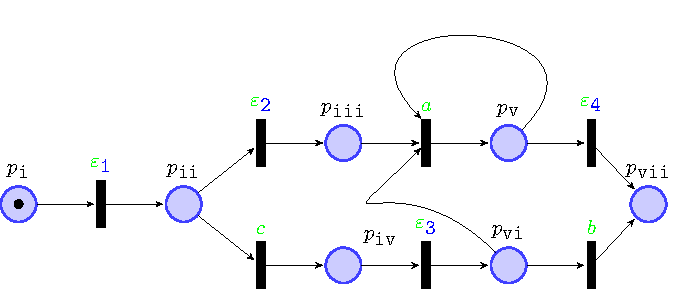
\includegraphics[width=.48\textwidth]{images/petri.pdf}}\hfill
    \subfloat[Reachability Graph of the \uswn in (a). Probabilities are shown in violet.]{\label{fig:rg}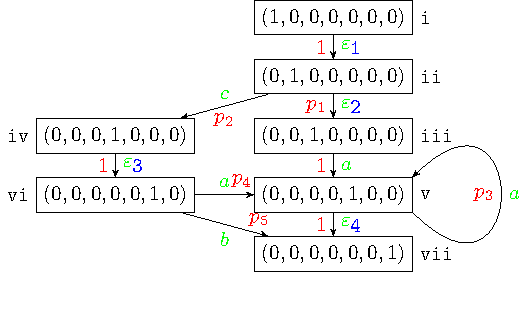
\includegraphics[width=.48\textwidth]{images/rg.pdf}}\\
	\subfloat[Reachability Graph Transformed as a Transition Graph.]{\label{fig:lmc}\label{fig:orig}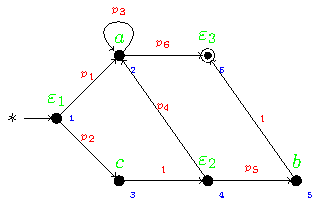
\includegraphics[width=.45\textwidth,trim=-1.2cm 0cm -1.2cm 0cm]{images/running_example.pdf}} \hfill 
	\subfloat[Transition Graph after $\varepsilon$-closure.]{\label{fig:closed}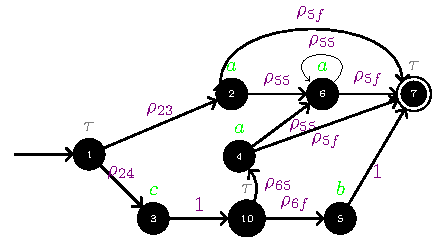
\includegraphics[width=.45\textwidth]{images/closed_example.pdf}}
	\caption{An \uswn and the application of the three transformation steps to convert it into a minimal, trace-preserving transition graph.}
	\label{transformspn}
\end{figure}
Figures \ref{fig:spn} and \ref{fig:rg} show a sample \uswn and its corresponding reachability graph, respectively. This net will be our running example throughout the paper.


%\begin{example}
%Figure \ref{fig:spn} provides a sample \uswn defined as such, and \ref{fig:rg} provides its associated Reachability Graph. This representation can be beneficial when such USWNs are inferred and extracted from log files \cite{PPNFromLog} for extracting the set of the probabilistic traces associated to the USWN.
%\end{example}
%
%
%We use USWNs for modelling business processes: in fact, it can be shown \cite{RaedtsPUWGS07} that it is always possible to convert BPMNs to USWNs. Last, we also assume that a transition is enabled when all of its input places contain at least one token and that, when a transition fires, we remove one token from each of its input places and depose tokens for each of its output places.



\subsection{Transition Graphs (TGs)}\label{subsec:ppn}
Current graph and trace embedding methods use a different graph representation, where nodes (and not edges) are labelled, 
and edges are still associated to a transition probability value.

Given finite sets $\Sigma$ of labels and $V\subset \mathbb{N}$ of nodes,  a \emph{(Probabilistic) Transition Graph} 
$(s,t,L,R,\omega)$ \cite{GartnerFW03} is uniquely described by an initial node $s\in V$, an accepting node $t\in V$, its labels, 
and a {Markov Chain with transition matrix $R$. The label matrix is defined by $[L]_{{\color{green}\alpha}\texttt{\color{blue}i}}=1\Leftrightarrow {\color{green}\alpha}=\textit{label}(\texttt{\color{blue}i})$ and $[L]_{{\color{green}\alpha}\texttt{\color{blue}i}}=0$ otherwise, and the transition matrix is defined by the probability $[R]_{\texttt{\color{blue}ij}}$ that the process will, when in node $\texttt{\color{blue}i}$, make a transition into node $\texttt{\color{blue}j}$ \cite{Prob} with $\sum_{\texttt{\color{blue}j}\in V}[R]_{\color{blue}\texttt{ij}}=1$. $[R^n]_{\texttt{\color{blue}ij}}$ denotes the probability of having a path $\texttt{\color{blue}i}\overset{n}{\rightsquigarrow}\texttt{\color{blue}j}$ of length $n$: therefore, $[\Lambda^n]_{\color{green}\alpha\beta}:=[LR^nL^t]_{\color{green}\alpha\beta}/[LL^t]_{\color{green}\alpha\alpha}$ denotes the probability of reaching
from a node labelled $\color{green}\alpha$ a node labelled $\color{green}\beta$ in $n$ steps (${\color{green}\alpha}\overset{n}{\rightsquigarrow}{\color{green}\beta}$). We denote as ${\color{green}\alpha}{\rightsquigarrow}{\color{green}\beta}$ an aforementioned path of arbitrary length. 
We can also associate a weight $\omega\in[0,1]\subseteq\mathbb{R}$ to a TG, to express the probability associated with the TG itself as valid. We represent such TG as in \cite{Myers1989}.
%
 Given a TG $P=(s,t,L,R,\omega)$, a trace $\tau$ is a tuple in $(\Sigma\backslash\{\varepsilon\})^*$ denoting a path always originating from $s$ and terminating in $t$. 


\begin{example} 
Figure \ref{fig:orig} is a  TG $P^*=(\mathtt{\color{blue}1},\mathtt{\color{blue}8},L,R,1)$ where $\omega=1$, where the matrices $L$ and $R$ can be both defined as follows:
$$L:=\kbordermatrix{
             & \texttt{\color{blue}1}&\texttt{\color{blue}2}&\texttt{\color{blue}3}&\texttt{\color{blue}4}&\texttt{\color{blue}5}&\texttt{\color{blue}6}&\texttt{\color{blue}7}&\texttt{\color{blue}8}&\texttt{\color{blue}9}&\texttt{\color{blue}10}\\
\color{green}\varepsilon  & \textbf{1}&0&0&0&0&0&\textbf{1}&\textbf{1}&\textbf{1}&\textbf{1}\\
\color{green}a            & 0&\textbf{1}&0&\textbf{1}&0&\textbf{1}&0&0&0&0\\
\color{green}b            & 0&0&0&0&\textbf{1}&0&0&0&0&0\\
\color{green}c            & 0&0&\textbf{1}&0&0&0&0&0&0&0\\
}\qquad \qquad
 R:=\kbordermatrix{
& \texttt{\color{blue}1}&\texttt{\color{blue}2}&\texttt{\color{blue}3}&\texttt{\color{blue}4}&\texttt{\color{blue}5}&\texttt{\color{blue}6}&\texttt{\color{blue}7}&\texttt{\color{blue}8}&\texttt{\color{blue}9}&\texttt{\color{blue}10}\\
\texttt{\color{blue}1}  & 0&0&{\color{violet}\pb}&0&0&0&0&0&{\color{violet}\pa}&0\\
\texttt{\color{blue}2}  & 0&0&0&0&0&{\color{violet}\pc}&{\color{violet}\pf}&0&0&0\\
\texttt{\color{blue}3}  & 0&0&0&0&0&0&0&0&0&{\color{violet}1}\\
\texttt{\color{blue}4}  & 0&0&0&0&0&{\color{violet}\pc}&{\color{violet}\pf}&0&0&0\\
\texttt{\color{blue}5}  & 0&0&0&0&0&0&0&{\color{violet}1}&0&0\\
\texttt{\color{blue}6}  & 0&0&0&0&0&{\color{violet}\pc}&{\color{violet}\pf}&0&0&0\\
\texttt{\color{blue}5}  & 0&0&0&0&0&0&0&{\color{violet}1}&0&0\\
\texttt{\color{blue}8}  & 0&0&0&0&0&0&0&0&0&0\\
\texttt{\color{blue}9}  & 0&{\color{violet}1}&0&0&0&0&0&0&0&0\\
\texttt{\color{blue}10}  & 0&0&0&{\color{violet}\pd}&{\color{violet}\pe}&0&0&0&0&0\\
}$$
\end{example}

\subsection{Kernels and Trace Kernels}\label{subsec:katk}
Given a set of data examples $\mathcal{X}$, (e.g., string or traces, TGs) a (positive definite) \textbf{kernel} function 
$k\colon \mathcal{X}\times \mathcal{X}\to \mathbb{R}$ denotes the similarity of elements in $\mathcal{X}$. If $\mathcal{X}$ is the $d$-dimensional Euclidean Space $\mathbb{R}^d$, the simplest kernel function is the inner product 
$\Braket{\mathbf{x},\mathbf{x}'}=\sum_{1\leq i\leq d}\mathbf{x}_i\mathbf{x}'_i$. 
A kernel \textbf{performs ideally} if $k(x,x')=1\Leftrightarrow x=x'$ (\textit{strong equality}) and 
$k(x,x')=0\Leftrightarrow x\not\simeq x'$ (\textit{strong dissimilarity}) \cite{Gartner03}. It is \textbf{appropriate} when similar 
elements $x,x'\in\mathcal{X}$ appear close in the feature space; this can only be assessed  empirically \cite{Gartner03}.
Any positive definite kernel induces a distance metric \cite{Raedt}:
\begin{equation}\label{eq:dofk}
d_k(\mathbf{x},\mathbf{x}'):=\sqrt{k(\mathbf{x},\mathbf{x})-2k(\mathbf{x},\mathbf{x}')+k(\mathbf{x}',\mathbf{x}')}
\end{equation}
When the kernel is the inner product, the resulting distance is the Euclidean distance $\norm{\mathbf{x}-\mathbf{x}'}{2}$. 
A normalized vector (versor) $\hat{\mathbf{x}}$ is defined as $\mathbf{x}/\norm{\mathbf{x}}{2}$: we can easily prove for normalized vectors that $\norm{\hat{\mathbf{x}}-\hat{\mathbf{x}}'}{2}^2=2(1-\Braket{\hat{\mathbf{x}},\hat{\mathbf{x}}'})$.
%
If $\mathcal{X}$ does not represent a $d$-dimensional Euclidean space, we can use an \textbf{embedding} 
$\phi\colon\mathcal{X}\to \mathbb{R}^d$ to define a kernel $k_\phi\colon \mathcal{X}\times \mathcal{X}\to\mathbb{R}$ as $k_\phi(x,x'):=\Braket{\phi(x),\phi(x')}$. As a result, $k_\phi(x,x')=k_\phi(x',x)$ for each $x,x'\in\mathcal{X}$.

Kernel representations also exist for traces (or strings in Databases~\cite{LodhiSSCW02,Raedt,GartnerFW03}). We 
provide an intuition of the desired features of such representation: if we associate each dimension in $\mathbb{R}^d$ to a different subtrace ${\color{green}\alpha\beta}\in(\Sigma\backslash\{\varepsilon\})^2$ of size $2$ ($2$-grams\footnote{\label{fn:caveat}In our experiments, we consider only $2$-grams, but traces of any length $p\geq 2$ can be used \cite{Gartner03}. A larger $p$ increases precision to the detriment of efficiency, as all the arbitrary sequences of length $p$ occurring at distance $i<|\tau|$ must be considered.}), the associated coordinate represents how frequently and ``compatctly'' such subtrace is embedded in the original trace. Therefore, we need to introduce a \textbf{decay factor} $\lambda\in[0,1]\subseteq\mathbb{R}$ weighting the presence of each subtrace ``${\color{green}\alpha\beta}/L$'' as $\lambda^Lm$, where $m$ is the frequency of $\color{green}\alpha\beta$ appearing in the given trace at a distance $L$. Given a trace $\tau\in\Sigma^*$, we represent it as a TG \cite{Myers1989} $(1,{|\tau|},L_\tau,R_\tau,1)$ having $[L_\tau]_{{\color{green}\alpha}\texttt{\color{blue}i}}=1\Leftrightarrow \tau_{\texttt{\color{blue}i}}={\color{green}\alpha}$ and $[L_\tau]_{{\color{green}\alpha}\texttt{\color{blue}i}}=0$ otherwise, and $\forall i<|\tau|.\; [R_\tau]_{\texttt{\color{blue}i(i+1)}}=1 $ and $[R_\tau]_{\texttt{\color{blue}ij}}=0$ otherwise. 
We can thus simplify the definition of the embedding from \cite{LodhiSSCW02,Raedt} as 
$\phi_{\mathcal{T}}(\tau)_{{\color{green}\alpha\beta}}=\sum_{1\leq i\leq |\tau|}\lambda^i[(\Lambda_\tau)^i]_{\color{green}\alpha\beta}$. 
Note that this definition is similar to a transition matrix embedding proposed in \cite{GartnerFW03} via geometric series: 
$\sum_i\lambda^i[R^i]_{\color{green}\alpha\beta}$. 

\begin{figure}[!t]
	\centering
	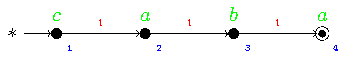
\includegraphics{images/taustar.pdf}
	\caption{Graphical representation of $\tau^*=\textup{caba}$ as a Thompson automaton.}\label{fig:taustar}
\end{figure}
\begin{example}\label{ex:tracembed}
	{Suppose that we want to align a trace $\tau^*=\textup{caba}$ (Figure \ref{fig:taustar}) to one of the traces from a TG. 
	For an approximate alignment, we need to transform $\tau^*$ to a TG first.} The associated TG 
	$T=(\mathtt{\color{blue}1},\mathtt{\color{blue}4},L,R,1)$ is given by:
	$$L:=\kbordermatrix{
		& \texttt{\color{blue}1}&\texttt{\color{blue}2}&\texttt{\color{blue}3}&\texttt{\color{blue}4}\\
		\color{green}a            & 0&\textbf{1}&0&\textbf{1}\\
		\color{green}b            & 0&0&\textbf{1}&0\\
		\color{green}c            & \textbf{1}&0&0&0\\
	}\qquad R:=\kbordermatrix{
		& \texttt{\color{blue}1}&\texttt{\color{blue}2}&\texttt{\color{blue}3}&\texttt{\color{blue}4}\\
		\texttt{\color{blue}1}  & 0&\color{violet}1&0&0\\
		\texttt{\color{blue}2}  & 0&0&\color{violet}1&0\\
		\texttt{\color{blue}3}  & 0&0&0&\color{violet}1\\
		\texttt{\color{blue}4}  & 0& 0& 0& 0\\
	}$$
We can similarly represent all the traces from the \uswn.
\end{example}

%\begin{example}
%The subtrace \textit{\textbf{\uline{hi}}} is represented in \textit{\textbf{\uline{hi}}deous},   \textit{\uline{\textbf{h}}e\uline{{i}}d\textbf{i}}, and \textit{\uline{{\textbf{h}i}}nd\textbf{i}}, but with different frequencies and subtrace distances. We have $\phi_{\mathcal{T}}(\textit{hideous})_{{\color{green}hi}}=\lambda$,  $\phi_{\mathcal{T}}(\textit{heidi})_{{\color{green}hi}}=\lambda^2+\lambda^4$, and $\phi_{\mathcal{T}}(\textit{hindi})_{{\color{green}hi}}=\lambda+\lambda^4$.
%\end{example}



\begin{table}[!t]
\caption{Embedding for both $\tau^*=cacb$ and some traces caaa, caa and cb generated from the USPN $\mathcal{U}$ in Figure \ref{fig:spn}}\label{tb:embedding}
\begin{center}
	\begin{tabular}{l@{\quad }l@{\quad }l@{\quad }l@{\quad }l@{\quad }l@{\quad }l@{\quad }l@{\quad }l@{\quad }l}
		\toprule
		& aa    & ab   & ac    & ba   & bb   & bc & ca & cb & cc   \\
		\midrule
		cacb & $0$ & $\lambda^2$ & $\lambda$ & $0$  & $0$  & $0$ & $\lambda$ & $\lambda+\lambda^3$ & $\lambda^2$\\
		caaa & $2\lambda+\lambda^2$& $0$ & $0$ & $0$ & $0$ & $0$ & $\lambda+\lambda^2+\lambda^3$ & $0$ & $0$ \\
		caa  & $\lambda$ & $0$ & $0$ & $0$ & $0$ & $0$ & $\lambda+\lambda^2$ & $0$&  $0$\\
		cb   & $0$ & $0$ & $0$ & $0$ & $0$ & $0$ & $0$ & $\lambda$& $0$ \\
		\bottomrule
	\end{tabular}
\end{center}
\end{table}
\begin{example}\label{ex:wheredotiszero}
Given $\Sigma_\varepsilon=\{a,b,c\}$, $\Sigma^2_\varepsilon=\{aa,ab,ac,ba,bb,bc,ca,cb,cc\}$ is the set of all $2$-grams 
from $\Sigma_\varepsilon$ induced by the non-$\varepsilon$ transitions within the \uswn $\mathcal{U}$ in Figure \ref{fig:spn}. 
For each $2$-gram ${\color{green}\alpha\beta}\in\Sigma_\varepsilon^2$ in a given trace $\tau$, we have a non-zero component 
$\phi_{\mathcal{T}}(\tau)_{\color{green}\alpha\beta}$ describing a penalty \cite{Gartner03}, while the kernel between two 
traces is the sum of such penalties. Given a trace $cb$ associated to $\mathcal{U}$,  the only non-zero component of 
$\phi_{\mathcal{T}}(cb)$ is $cb$ itself, where $\phi_{\mathcal{T}}(cb)_{\color{green}cb}=\lambda$ (Table \ref{tb:embedding}). 
On the other hand, the trace $caa$ from $\mathcal{U}$ has a $2$-gram $ca$ with occurring lengths $1$ (\textbf{ca}a) and $2$ (\textbf{c}a\textbf{a}), and $aa$ with occurring length $1$; therefore, $\phi_{\mathcal{T}}(caa)_{\color{green}ca}=\lambda+\lambda^2$ and  $\phi_{\mathcal{T}}(caa)_{\color{green}aa}=\lambda$.  Similar considerations can be carried out for the other traces cacb and caaa, whose embeddings are represented in Figure \ref{tb:embedding}. 

Evaluating the similarity between $\tau^*=cacb$ and the other traces, we obtain: 
$k_{\phi_{\mathcal{T}}}(cacb,caaa)=\lambda(\lambda+\lambda^2+\lambda^3)$,  
$k_{\phi_{\mathcal{T}}}(cacb,caa)=\lambda(\lambda+\lambda^2)$, 
and $k_{\phi_{\mathcal{T}}}(cacb,cb)=\lambda(\lambda+\lambda^3)$, yielding the ranking $k_{\phi_{\mathcal{T}}}(cacb,caaa)>k_{\phi_{\mathcal{T}}}(cacb,caa)>k_{\phi_{\mathcal{T}}}(cacb,cb)$. For this trace kernel, we have strong dissimilarity when the two traces have no shared $2$-grams at any arbitrary occurring length ($k_{\phi_{\mathcal{T}}}(caa,cb)=0$) but no strong equality ($k_{\phi_{\mathcal{T}}}(cb,cb)=\lambda^2$ with $\lambda^2\neq 1$ for $0\leq \lambda<1$).
\end{example}

\subsection{Graph Embedding}\label{ssec:ge}
Graph kernels map graph data structures to feature spaces (usually an Eulcidean space) to express graph similarity functions 
that can be adopted for classification \cite{TsudaS10} and clustering \cite{Raedt} algorithms. One of the first approaches used 
\cite{Sidere} involved the definition of topological description vectors for each graph in a graph database, and defining the graph 
similarity function as an inner product of their associated vectors. One inconvenience of this technique is that it is required to 
perform NP-complete subgraph isomorphisms among a collection of graphs. It has been already proved that the definition of a 
graph kernel function fully recognising the structure the graph always boils down solving such  NP-Complete problem 
\cite{GartnerFW03}, as exact embeddings generable in polynomial can be inferred just for loop-free DAGs \cite{BergamiBM20}.  
%
Consequently, most recent methods focus on extracting relevant features of graphs, which are used to define a similarity function. 
The most common approach adopted is called \textit{propositionalisation}: extract all the possible features (e.g., 
subsequences), and define a kernel function based on the occurrence and similarity of these features \cite{Gartner03}. 

%\section{LTL over Finite Traces and the Declare Framework}
%\label{sec:preliminaries}
%As a formal basis for specifying crisp (temporal) business constraints, we adopt the customary choice of Linear Temporal Logic over finite traces (\LTLf \cite{DeVa13,DDGM14}). This logic is at the basis of the well-known \declare \cite{PeSV07} constraint-based process modeling language.
%We provide here a gentle introduction to this logic and to the \declare framework.
%
%\subsection{Linear Temporal Logic over Finite Traces}
%
%$\LTLf$ has exactly the same syntax as standard $\LTL$, but, differently from $\LTL$, it interprets formulae over an unbounded, yet finite linear sequence of states. Given an alphabet $\Sigma$ of atomic propositions (in our setting, representing activities), an \LTLf formula $\varphi$ is built by extending propositional logic with temporal operators:
%\[\varphi ::= a \mid \lnot \varphi \mid \varphi_1\lor \varphi_2
% \mid \Next\varphi \mid \varphi_1\Until\varphi_2 \quad \text{ where $a \in \Sigma$.}\]
%
%
%%The semantics of \LTLf is given in terms of \emph{finite traces}
%%denoting finite, \emph{possibly empty}, sequences
%%$\tau=\tau_0,\ldots,\tau_n$ of elements from the alphabet $\Sigma$. The evaluation of a formula is done in a given state (i.e., position) of the trace.
%
%
%The semantics of \LTLf is given in terms of \emph{finite traces} denoting finite, \emph{possibly empty} sequences $\tau=\tup{\tau_0, \ldots, \tau_n}$ of elements of $2^\Sigma$, containing all possible propositional interpretations of the propositional symbols in $\Sigma$. In the context of this paper, consistently with the literature on business process execution traces, we make the simplifying assumption that in each point of the sequence, one and only one element from $\Sigma$ holds. Under this assumption, $\tau$ becomes a total sequence of activity occurrences from $\Sigma$, matching the standard notion of (process) execution trace. We indicate with $\tasks^*$ the set of all traces over $\tasks$. The evaluation of a formula is done in a given state (i.e., position) of the trace, and we use the notation $\tau,i\models \varphi$ to express that $\varphi$ holds in the position $i$ of $\tau$. We also use $\tau \models \varphi$ as a shortcut notation for $\tau,0\models\varphi$. This denotes that $\varphi$ holds over the entire trace $\tau$ starting from the very beginning and, consequently, logically captures the notion of \emph{conformance} of $\tau$ against $\varphi$. We also say that $\varphi$ is \emph{satisfiable} if it admits at least one conforming trace.
%
%%We start by giving an intuitive account of the resulting semantics. In the syntax above, operator $\Next$ denotes the \emph{next state} operator, and $\Next \varphi$ is true if $\varphi$ is true is true now if there exists a next state (i.e., the current state is not at the end of the trace), and in the next state $\varphi$ holds. Operator $\Until$ instead is the \emph{until} operator, and $\varphi_1\Until\varphi_2$ is true if $\varphi_1$ holds now and continues to hold until eventually, in a future state, $\varphi_2$ holds. From the given syntax we can derive the usual boolean operators $\land$ and $\rightarrow$, the two formulae $\true$ and $\false$, as well also additional temporal operators. We consider in particular the following three:
%%\begin{compactitem}[$\bullet$]
%%\item (eventually) $\Diamond \varphi = \true \Until \varphi$ is true if there is a future state where $\varphi$ holds;
%%\item (globally) $\Box \varphi = \neg \Diamond \neg \varphi$ is true if now and in all future sates $\varphi$ holds;
%%\item (weak until) $\varphi_1 \Wntil \varphi_2 = \varphi_1\Until\varphi_2 \lor \Box \varphi_1$ relaxes the until operator by admitting the possibility that $\varphi_2$ never becomes true, in this case by requiring that is true if $\varphi_1$ holds now and in all future states.
%%\end{compactitem}
%% To define the semantics formally, we denote the length of trace $\tau$ as $\length(\tau) =  n+1$.
%
%
%In the syntax above, operator $\Next$ denotes the \emph{next state} operator, and $\Next \varphi$ is true if there exists a next state (i.e., the current state is not at the end of the trace), and in the next state $\varphi$ holds. Operator $\Until$ instead is the \emph{until} operator, and $\varphi_1\Until\varphi_2$ is true if $\varphi_1$ holds now and continues to hold until eventually, in a future state, $\varphi_2$ holds. From these operators, we can derive the usual boolean operators $\land$ and $\rightarrow$, the two formulae $\true$ and $\false$, as well as additional temporal operators. We consider, in particular, the following three:
%\begin{compactitem}[$\bullet$]
%\item (eventually) $\Diamond \varphi = \true \Until \varphi$ is true if there is a future state where $\varphi$ holds;
%\item (globally) $\Box \varphi = \neg \Diamond \neg \varphi$ is true if now and in all future states $\varphi$ holds;
%\item (weak until) $\varphi_1 \Wntil \varphi_2 = \varphi_1\Until\varphi_2 \lor \Box \varphi_1$ relaxes the until operator by admitting the possibility that $\varphi_2$ never becomes true, in this case by requiring that $\varphi_1$ holds now and in all future states.
%\end{compactitem}
%%We write $\tau \models \varphi$ as a shortcut notation for $\tau,0\models \varphi$, and say that formula $\varphi$ is \emph{satisfiable}, if there exists a trace $\tau$ such that $\tau \models \varphi$.
%
%\begin{example}
%The $\LTLf$ formula $\Box(\activity{accept} \rightarrow \Diamond\activity{pay})$ models that, whenever an order is accepted, then it is eventually paid. The structure of the formula follows what is called \emph{response template} in \declare.
%\end{example}
%
%%Every $\LTLf$ formula $\varphi$ can be translated into a corresponding standard finite-state automaton $\aut_\varphi$ that accepts all and only those finite traces that satisfy $\varphi$ \cite{DeVa13,DDGM14}. Although the complexity of reasoning with $\LTLf$ is the same as that of $\LTL$, finite-state automata are much easier to manipulate in comparison with B\"uchi automata, which are necessary when formulae are interpreted over infinite traces.
%
%\subsection{Declare}
%\begin{table}[t]
\caption{Some \declare templates, their textual and graphical representation, the corresponding \LTLf formalization and the \LTLf formula capturing their complement (i.e., their logical negation).
\label{tab:constraints}}
\centering
\begin{adjustbox}{width=0.9\textwidth,center}
\begin{tikzpicture}
  \matrix[  nodes={node distance=\nodedist,minimum height=6mm},
            rectangle, draw,
            nodes in empty cells,
            row sep=2mm,column sep=3mm,
            very thick,
            column 1/.style={anchor=west,font=\footnotesize},
            column 2/.style={anchor=west,xshift=1mm,font=\footnotesize},
            column 3/.style={anchor=west,xshift=1mm,font=\footnotesize},
            column 4/.style={anchor=west},
            >=latex,->,
          ] (declarematrix) {
    \node {\textsc{text}};
    &
    \node[yshift=.5mm] {\textsc{notation}};
  &
    \node {\textsc{\LTLf\ formula ($\varphi$)}};
    &
    \node[yshift=.5mm] {\textsc{complement ($\neg\varphi$)}};
    \\
    \node {
      \begin{tabular}{@{}l@{}}
      \constraint{existence($\mathit{a}$)} \\
      \end{tabular}
    };
    &
    \node[smalltask,xshift=1.5mm] (a) {$\mathit{a}$};
    \node[taskfg,above=-1mm of a,xshift=-.3mm]{\footnotesize $1..\ast$};
    &
    \node {$\Diamond {a}$};
    &
    \node {$\Box \neg {a}$};

    \\
     \node {
      \begin{tabular}{@{}l@{}}
        \constraint{absence2($\mathit{a}$)}\\
      \end{tabular}
    };
    &
    \node[smalltask,xshift=1.5mm] (a) {$\mathit{a}$};
    \node[taskfg,above=-1mm of a,xshift=-.3mm]{\footnotesize $0..1$};

    &
    \node {$\neg \Diamond ({a} \land \Next \Diamond {a})$};
    &
    \node {$\Diamond ({a} \land \Next \Diamond {a})$};
    \\
    \node {
      \begin{tabular}{@{}l@{}}
        \constraint{response($\mathit{a}$,$\mathit{b}$)}
      \end{tabular}
    };
    &
    \node[smalltask,xshift=1.5mm] (a) {$\mathit{a}$};
    \node[above=-1mm of a,xshift=-.3mm]{\footnotesize $~$};
    \node[smalltask,right=\taskdist of a] (b) {$\mathit{b}$};
    \path[response,very thick] (a) -- (b);
    &
    \node {$\Box ({a} \rightarrow \Diamond {b})$};
    &
    \node {$\Diamond ({a} \land \Box \neg {b})$};
    \\
    \node {
      \begin{tabular}{@{}l@{}}
        \constraint{precedence($\mathit{a}$,$\mathit{b}$)}\\
      \end{tabular}
    };
    &
    \node[smalltask,xshift=1.5mm] (a) {$\mathit{a}$};
    \node[smalltask,right=\taskdist of a] (b) {$\mathit{b}$};
    \path[precedence,very thick] (b) -- (a);
    &
    \node {$\neg {b} \Wuntil {a}$};
    &
    \node {$\neg {a} \Until {b}$};
    \\
    \node {
      \begin{tabular}{@{}l@{}}
        \constraint{not-coexistence($\mathit{a}$,$\mathit{a}$)}\\

      \end{tabular}
    };
    &
    \node[smalltask,xshift=1.5mm] (a) {$\mathit{a}$};
    \node[smalltask,right=\taskdist of a] (b) {$\mathit{b}$};
    \path[notcoexistence,very thick] (a) -- (b);
    &
    \node {$\neg(\Diamond {a} \land \Diamond {b})$};
    &
    \node {$\Diamond {a} \land \Diamond {b}$};
    \\
%    \node {
%      \begin{tabular}{@{}l@{}}
%        \constraint{neg-response(\activity{a},\activity{b})}\\
%        $\Box( \activity{a} \limp \neg \bigcirc\Diamond \activity{b})$
%      \end{tabular}
%    };
%    &
%    \node[smalltask,xshift=1.5mm] (a) {\activity{a}};
%    \node[smalltask,right=\taskdist of a] (b) {\activity{b}};
%    \path[negationresponse,very thick] (a) -- (b);
%    \\
    };
\end{tikzpicture}
\end{adjustbox}
\end{table} 
%\declare\ \cite{PeSV07} is a declarative process modeling language based on \LTLf. More specifically, a \declare model fixes a set of activities, and a set of constraints over such activities, formalized using \LTLf formulae. The overall model is then formalized as the conjunction of the \LTLf formulae of its constraints.
%
%Among all possible \LTLf formulae, \declare selects some pre-defined patterns. Each pattern is represented as a \declare template, i.e., a formula with placeholders to be substituted by concrete activities to obtain a constraint. Constraints and templates have a graphical representation; Table~\ref{tab:constraints} lists the \declare templates used in this paper. A \declare model is then graphically represented by showing its activities, and the application of templates to such activities (which indicates how the template placeholders have to be substituted to obtain the corresponding constraint).
%
%%Automata-based techniques for $\LTLf$ have been adopted to tackle fundamental tasks within the lifecycle of \declare processes, such as consistency checking \cite{PeSV07,MPVC11}, enactment and monitoring \cite{PeSV07,MMWV11,DDGM14}, and discovery support \cite{MaCV12}.
%
%
%
%
%\begin{example}
%\label{ex:inconsistency}
%Consider the following \declare model, constituting a (failed) attempt of capturing a fragment of an order-to-shipment process:
%
%\begin{center}
%  \resizebox{3.2cm}{!}{
%        \begin{tikzpicture}
%        \node[task] (accept) {\accept};
%        \node[task,right=of accept] (reject) {\reject};
%        \node[left=0mm of accept,taskfg] {1..*};
%        \node[right=0mm of reject,taskfg] {1..*};
%        \draw[notcoexistence] (accept) -- (reject);
%    \end{tikzpicture}
%  }
%\end{center}
%
%The model indicates that there are two activities to accept or reject an order, that these two activities are mutually exclusive, and that both of them have to be executed.
%%  \begin{wrapfigure}[13]{l}{42mm}
%%  \end{wrapfigure}
%These constraints are obviously contradictory and, in fact, the model is inconsistent, since its \LTLf formula
%$
%\Diamond \accept \land \Diamond \reject \land \neg (\Diamond \accept \land \Diamond \reject)
%$
%is unsatisfiable.
%\end{example}
%
%
%
%\endinput
%
%\smallskip\noindent\textbf{\declare} is a constraint-based process modeling language based on \LTLf. Differently from imperative process modeling languages,
%\declare models a process by fixing a set of activities, and defining a set of
%\emph{temporal constraints} over them, accepting every execution trace that satisfies all constraints.
%Constraints are specified via pre-defined \LTLf templates, which come with a corresponding
%graphical representation (see Table~\ref{tab:constraints} for the \declare patterns we use in this paper).
%For the sake of generality, in this paper we consider arbitrary \LTLf formulae as constraints. However, in the examples we consider formulae whose templates can be represented graphically in \declare.
%
%
%
%Automata-based techniques for $\LTLf$ have been adopted in \declare to tackle fundamental tasks within the lifecycle of Declare processes, such as consistency checking \cite{PeSV07,MPVC11}, enactment and monitoring \cite{PeSV07,MMWV11,DDGM14}, and discovery support \cite{MaCV12}.
